\documentclass{IEEEtran}
\usepackage[utf8]{inputenc}
\usepackage[alsoload=synchem,load=named]{siunitx}
\usepackage{graphicx}
\usepackage{amsmath}
\usepackage{booktabs, tabularx}
\usepackage{hyperref}
\usepackage{listings}
\usepackage{physics}
\usepackage[citestyle=ieee,sorting=none,bibencoding=utf8,backend=biber]{biblatex}

\graphicspath{{images/}}
\bibliography{bibliography}

\author{J.R. Powers-Luhn}
\title{Application of Simple Regression Models to Body Composition Measurements}
\date{September 25th, 2018}

\DeclareSIUnit\year{yr}
\DeclareSIUnit\inch{in}

\begin{document}
\maketitle

\begin{abstract}

A dataset of body composition measurements is used to explore linear regression techniques. Several regression models are developed, predicting body fat percentage within 4\%, performing unfavorably compared to the work of Penrose, et al \cite{Penrose1985}. Attempts to achieve the accuracy claimed by Penrose, et al, (0.6\% for lean body weight) were unsuccessful, achieving an error of 4.37 with the predictors they report. The sensitivity of the model to the selection of training, testing, and validation data is briefly discussed.

\end{abstract}

\section{Introduction}

Measurements of body fat percentage are desirable as they may be good predictors of heart attack risk later in life \cite{HealthyBodyFat2000}\cite{Rimm1995}. Currently the most accurate methods to measure body fat percentage require accurate measurements of overall density \cite{statsEducation}. This can involve techniques as extreme as whole-body immersion in a pool of deuterated or tritiated water \cite{HealthyBodyFat2000}.

\subsection{Linear Regression}

In general, a linear regression seeks the coefficients $\vec{\alpha}$ which minimize the error on equation \eqref{eq:linear}:

\begin{equation}
	\mathbf{x} \vec{a} = \vec{y}
	\label{eq:linear}
\end{equation}

where $\mathbf{x}$ represents the measured inputs from which we seek to predict the output, $y$. We can determine the best values for $\alpha$ by choosing to minimize the difference between our predicted and true values as in equation \eqref{eq:error}, leading to equation \eqref{eq:intregression}.

\begin{align}
	E(\alpha) &= (\mathbf{x} \vec{\alpha} - \vec{y})^2 \label{eq:error} \\
	\dv{E}{\alpha} = 0 &= 2 (\mathbf{x} \vec{\alpha} - \vec{y}) \mathbf{x} \nonumber \\
	\mathbf{x} \vec{\alpha} \mathbf{x} &= \vec{y} \mathbf{x} \nonumber \\
	\mathbf{x}^{-1} \mathbf{x} \vec{\alpha} \mathbf{x} \mathbf{x}^{-1} &= \mathbf{x}^{-1} \vec{y} \mathbf{x} \mathbf{x}^{-1} \nonumber \\
	\vec{\alpha} &= \mathbf{x}^{-1} \vec{y}
	\label{eq:intregression}
\end{align}

In order to have a unique solution to this equation, $\mathbf{x}$ must have at least as many rows as it has columns. In practice, the number of samples (rows) and the dimensionality of each sample (columns) are not linked to each other. In the case of the dataset examined in this paper, for example, there are many times more samples (247) than there are dimensions (14). In order to simplify this process, we therefore multiply $\mathbf{x}$ in equation \eqref{eq:linear} by its transpose $\mathbf{x}^T$ in order to obtain equation \eqref{eq:regression}.

\begin{align}
	\vec{\alpha} = (\mathbf{x}^T \mathbf{x})^{-1} \mathbf{x}^T \vec{y}
	\label{eq:regression}
\end{align}

Since the relationship between two quantities will not in general have a zero intercept, new ``input'' is added to the measured values prior to the regression. This input consists of a column of non-varying values (ones) which allows for the last element of $\alpha$ to correspond to the axis intercept when all inputs are zero.

\subsection{Solution Stability and Covariance}

Another complication arises in practice. In order to solve \eqref{eq:linear}, it is necessary to have at least as many \textit{linearly independent} rows as there are columns. In the event that some of the measured inputs covary, the solution becomes unstable and can vary wildly based on the noise in the sampled data. It may be desirable, therefore, to leave some sampled values out of the matrix in favor of others which capture the same information. A useful tool to choose variables to eliminate from consideration is the \textit{covariance matrix} or its normalized cousin, the \textit{correlation matrix}. 

The covariance of two variables is calculated using equation \eqref{eq:covariance}.

\begin{equation}
	cov(\vec{x}, \vec{y}) = \frac{1}{N-1} \sum^N_{i=1} (x_i - \bar{x}) (y_i - \bar{y})
	\label{eq:covariance}
\end{equation}

It is difficult to compare the covariance across the entire dimensionality of a dataset since the units are expected to differ. Therefore the more commonly employed value is the correlation (equation \eqref{eq:correlation}).

\begin{equation}
	corr(\vec{x}, \vec{y}) = \frac{cov(\vec{x}, \vec{y})}{\sigma_x \sigma_y}
	\label{eq:correlation}
\end{equation}

\subsection{Linear in parameters}

Of course, often the variable which is to be predicted does not depend linearly on the input variables--for example, square or higher-order polynomial terms (an example is shown in equation \eqref{eq:example_linear_in_parameters}).

\begin{equation}
	y = \alpha_1 x_1 + \alpha_2 x_1^2 + \alpha_3 x_2 + \alpha_4 x_1 x_2
	\label{eq:example_linear_in_parameters}
\end{equation}

In such a case it is still possible to fit the model using equation \eqref{eq:regression}. New ``inputs'' are created to take the non-linear terms \eqref{eq:linear_in_parameters2}. The coefficients can then be calculated.

\begin{align}
	&y = \alpha_1 x_1 + \alpha_2 x_3 + \alpha_3 x_2 + \alpha_4 x_4 \nonumber \\
	&x_3 = x_1^2 \nonumber \\
	&x_4 = x_1 x_2 \nonumber \\
	\label{eq:linear_in_parameters2}
\end{align}

While this technique does not work if the equation cannot be parameterized (e.g. $y=\sin(\alpha x)$), it can allow for the fitting of more complex datasets.

\subsection{Dataset examined}

The dataset analyzed was a subset of body measurements taken by Penrose\cite{Penrose1985}. This data set consists of 247 samples each of fourteen quantities:

\begin{itemize}
	\item Age (\si{\year})
	\item Weight (lbs)
	\item Height (inches)
	\item Adiposity index (\si{\kilo\gram\per\meter^2})
	\item Neck circumference (\si{\centi\meter})
	\item Chest circumference (\si{\centi\meter})
	\item Ab circumference (\si{\centi\meter})
	\item Hip circumference (\si{\centi\meter})
	\item Thigh circumference (\si{\centi\meter})
	\item Knee circumference (\si{\centi\meter})
	\item Ankle circumference (\si{\centi\meter})
	\item Extended bicep circumference (\si{\centi\meter})
	\item Forearm circumference (\si{\centi\meter})
	\item Wrist circumference (\si{\centi\meter})
\end{itemize}

\num{143} of these measured values were used to derive the lean body weight equation \eqref{eq:brozek}, with abdominal ($Ab$) and wrist ($Wr$) circumferences measured in \si{\centi\meter}, weight ($Wt$) measured in \si{\kilo\gram}, and height ($Hgt$) measured in \si{\meter}. This was then validated with \num{109} additional measurements.

\begin{multline}
	LBW = 17.298 + 0.89946 (Wt) - 0.2783 (Age) \\+ 0.002617 (Age^2) + 17.819 (Hgt) - 0.6798 (Ab - Wr) \label{eq:brozek}
\end{multline}

Outliers from the data were removed in order to provide a more representative analysis.

A variety of regressions were performed on linear and non-linear combinations of these measured input variables. 

\section{Methodology} 

The data were split into three groups for the purposes of this analysis. All regression was performed on the \textbf{training} group. Peformance scores for each regression were calculated using the \textbf{testing} group, and final results were reported using the \textbf{validation} group. Since each sample corresponded to a single patient there was deemed to be no relationship between rows in the dataset. This meant that the set could be divided by shuffling the rows and selecting the first 60\% as training data, the second 20\% as testing data, and the remaining 20\% as validation data. Since these fractions did not match whole numbers of training rows, the floor of each fraction ($\frac{train rows}{total rows}$, $\frac{test rows}{total rows}$, $\frac{val rows}{total rows}$) was taken and the remaining rows added to the training set. Performance for each regression was calculated using the root mean squared error (RMSE) for that prediction \eqref{eq:rmse}, where $x_i$ and $y_i$ are from the test set and $\alpha$ is calculated from the training set.

\begin{equation}
	RMSE = \sqrt{\frac{1}{N} \sum_{i=0}^N{(x_i \alpha - y_i)^2} }
	\label{eq:rmse}
\end{equation}

In order to test the one-variable regression performance, each column was used to perform a regression and the performance of each regression on the testing set was calculated. Next, two-variable regressions were performed on every combination of two inputs. An additional regression was performed using all fourteen of the input variables.

A correlation matrix was computed for the input and output values in order to inform a ``best guess'' of factors to use in a linear model. The inputs were selected based on both their correlation to body fat percentage and their lack of correlation to each other. This model was constructed and its performance measured.

In order to test the performance of non-linear terms, inverse and quadratic combinations of the input variables were calculated and used to perform additional regressions. 

\section{Results}

The correlation matrix calculated on the training set revealed that most values were somewhat correlated with body fat percentage (>0.3), but only abdominal circumference and adiposity index were strongly correlated (>0.7). Age, height, and ankle circumference were uncorrelated (<0.3) with body fat. Forearm and wrist circumference were borderline (0.32 and 0.35, respectively). A representation of the complete correlation matrix is shown in figure \ref{fig:corr_matrix}.

\begin{centering}
\begin{figure}
\centering
\begin{center}
	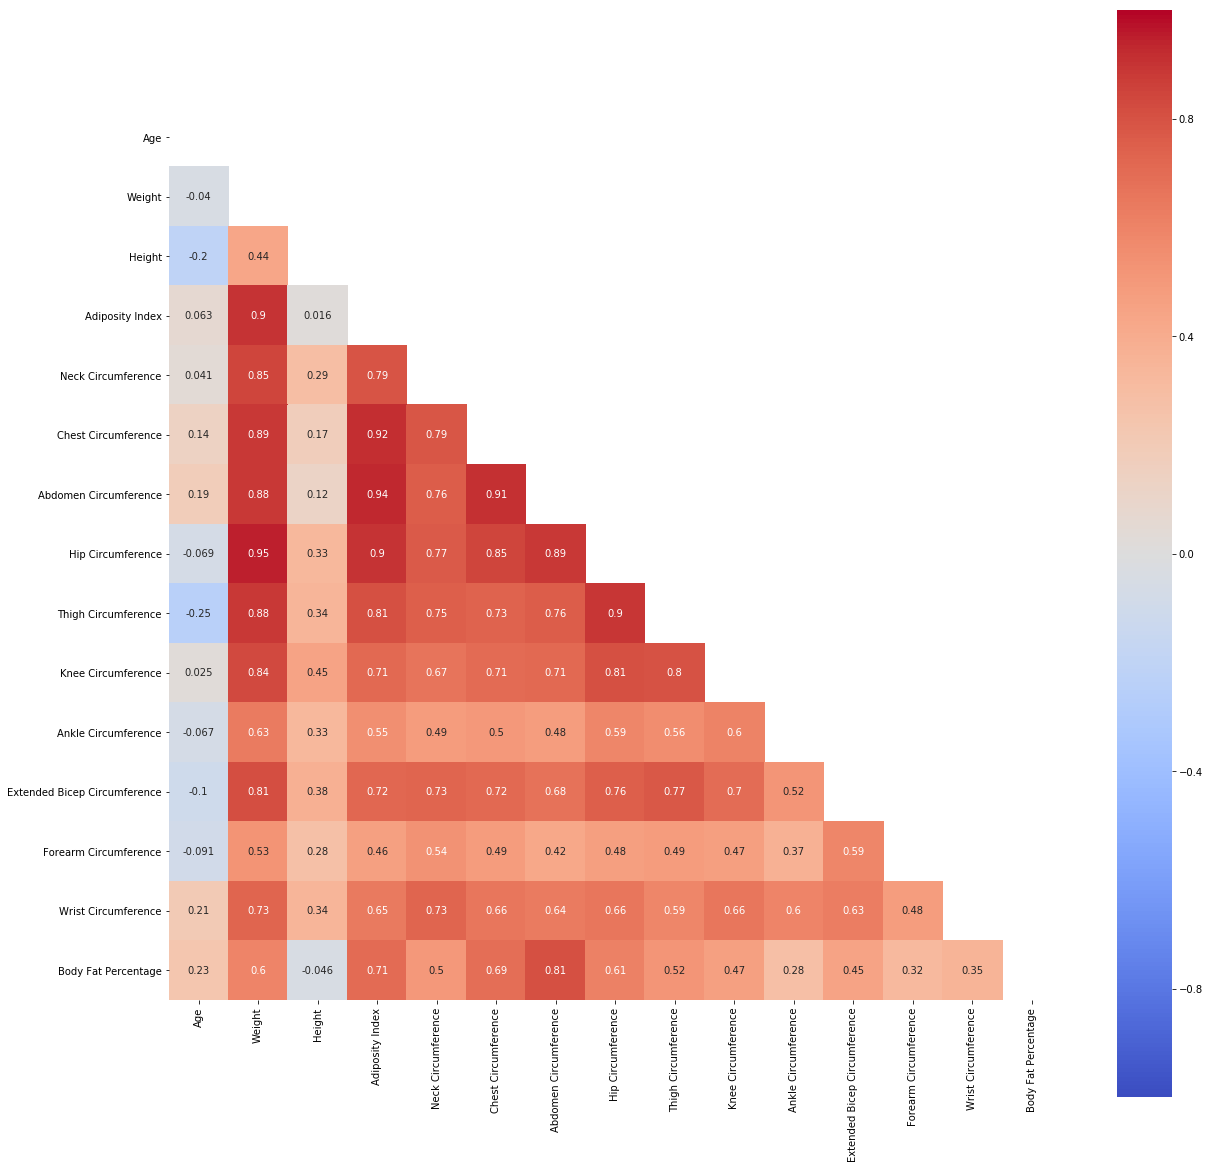
\includegraphics[width=0.5\textwidth]{corr_matrix}
	\caption{Correlations between each pair of data. Darker colors represent more correlation. All values except height and age are positively correlated with each other.\label{fig:corr_matrix}}
\end{center}
\end{figure}
\end{centering}

Fourteen regressions were performed using a single column as input. The best single input was determined to be abdominal circumference based on its test error of 4.47. The single worst input was determined to be height with an error of 6.74. The validation performance of the abdominal circumference model was 4.14. The performance of all models on the test set can be seen in figure \ref{fig:one_var_perf}.

\begin{centering}
\begin{figure}
\centering
\begin{center}
	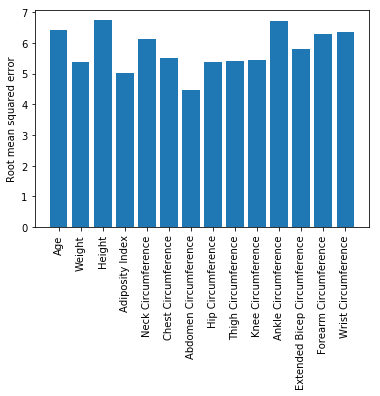
\includegraphics[width=0.5\textwidth]{one_var_perf}
	\caption{Performance of one-variable regression models on the test set as a function of input variable. The range of errors was 2.3 percentage points. Inputs with the highest correlation to the output were unsuprisingly higher performing.\label{fig:one_var_perf}}
\end{center}
\end{figure}
\end{centering}

The regressions against paired columns showed slightly better results. The performance of these models ranged from a minimum of 4.20 (abdomen circumference and wrist circumference) to a maximum of 6.84 (height and ankle circumference). Validation performance of the best model produced an RMSE of 4.07. While wrist circumference was particularly uncorrelated with body fat percentage, it is theorized that including it in this model improved performance because it was also uncorrelated with abdomen circumference and thus contained information not captured in the abdomen circumference value alone. Height was also uncorrelated with abdomen circumference and body fat percentage, but the model that included abdomen circumference and height had a validation error of only 3.67. This suggests that choosing variables based on their orthogonality and not simply correlation can have a positive effect on a model.

Regression against the entire range of fourteen inputs produced performance on the test set with an RMSE of 4.55, but it fared quite a bit better on the validation set (3.75). This trend was followed by the ``best guess'' regression against abdomen circumference, wrist circumference, and height, whose performance on the validation set (3.83) was also better than the performance on the test set (4.14).

Based on the theory that body fat percentage should be inversely correlated with weight, a regression was performed against abdomen circumference, height, and wrist circumference with the addition of $\frac{1}{weight}$. This theory was not born out, with a test error of 4.11 but a validation error of 3.87, performing approximately as well as the ``best guess'' regression.

While it would not be appropriate to choose a model based on the results of the validation set, the swings in accuracy between test and validation performance indicate that the statistics of their respective data sets may be different. Based on the small variation in accuracy when comparing these models, it is not possible to select a ``best'' model from the data presented in this paper. 

A comparison was made of the errors presented to the standard deviation of body fat percentage in the training set. The standard deviation of body fat percentage in the training set was 7.88. This means that the model which performed the best on the test set (abdomen and wrist circumference, height, $weight^{-1}$) had a validation error of approximately 1/2 standard deviations. By contrast, the worst-performing single-variable regression (height) had a test error of 0.87 standard deviations.

\section{Conclusions}

Several models were generated, predicting body fat percentage from height, weight, and circumference measurments to an error of approximately 4\%. Performance measurements were limited to root mean squared error, but will be extended in the future to include variance in the error in an attempt to capture this. More sophisticated cross-validation techniques may be appropriate when examining datasets with high variance in their values. This data selection problem is one possible explanation of why the regression performed in this paper had such poor results when compared to that presented by Penrose, et al.

%\nocite{*}
\printbibliography

%\onecolumn
%\section{Appendix}
%Python code used to perform calculations and generate graphics.
%\lstset{frame=single}
%\lstinputlisting[language=python]{appendix/appendix.py}

\end{document}